\documentclass{exam}

\usepackage{siunitx} 
\usepackage{graphicx}
\usepackage[fleqn]{amsmath}
\usepackage{cancel}
\usepackage{float}
\usepackage{mdwlist}
\usepackage{booktabs}
\usepackage{cancel}
\usepackage{polynom}
\usepackage{caption}
\usepackage{fullpage}
\usepackage{comment}
\usepackage{enumerate}

\newcommand{\degree}{\ensuremath{^\circ}} 
\everymath{\displaystyle}

% \begin{figure}[H]
%   \centering
%   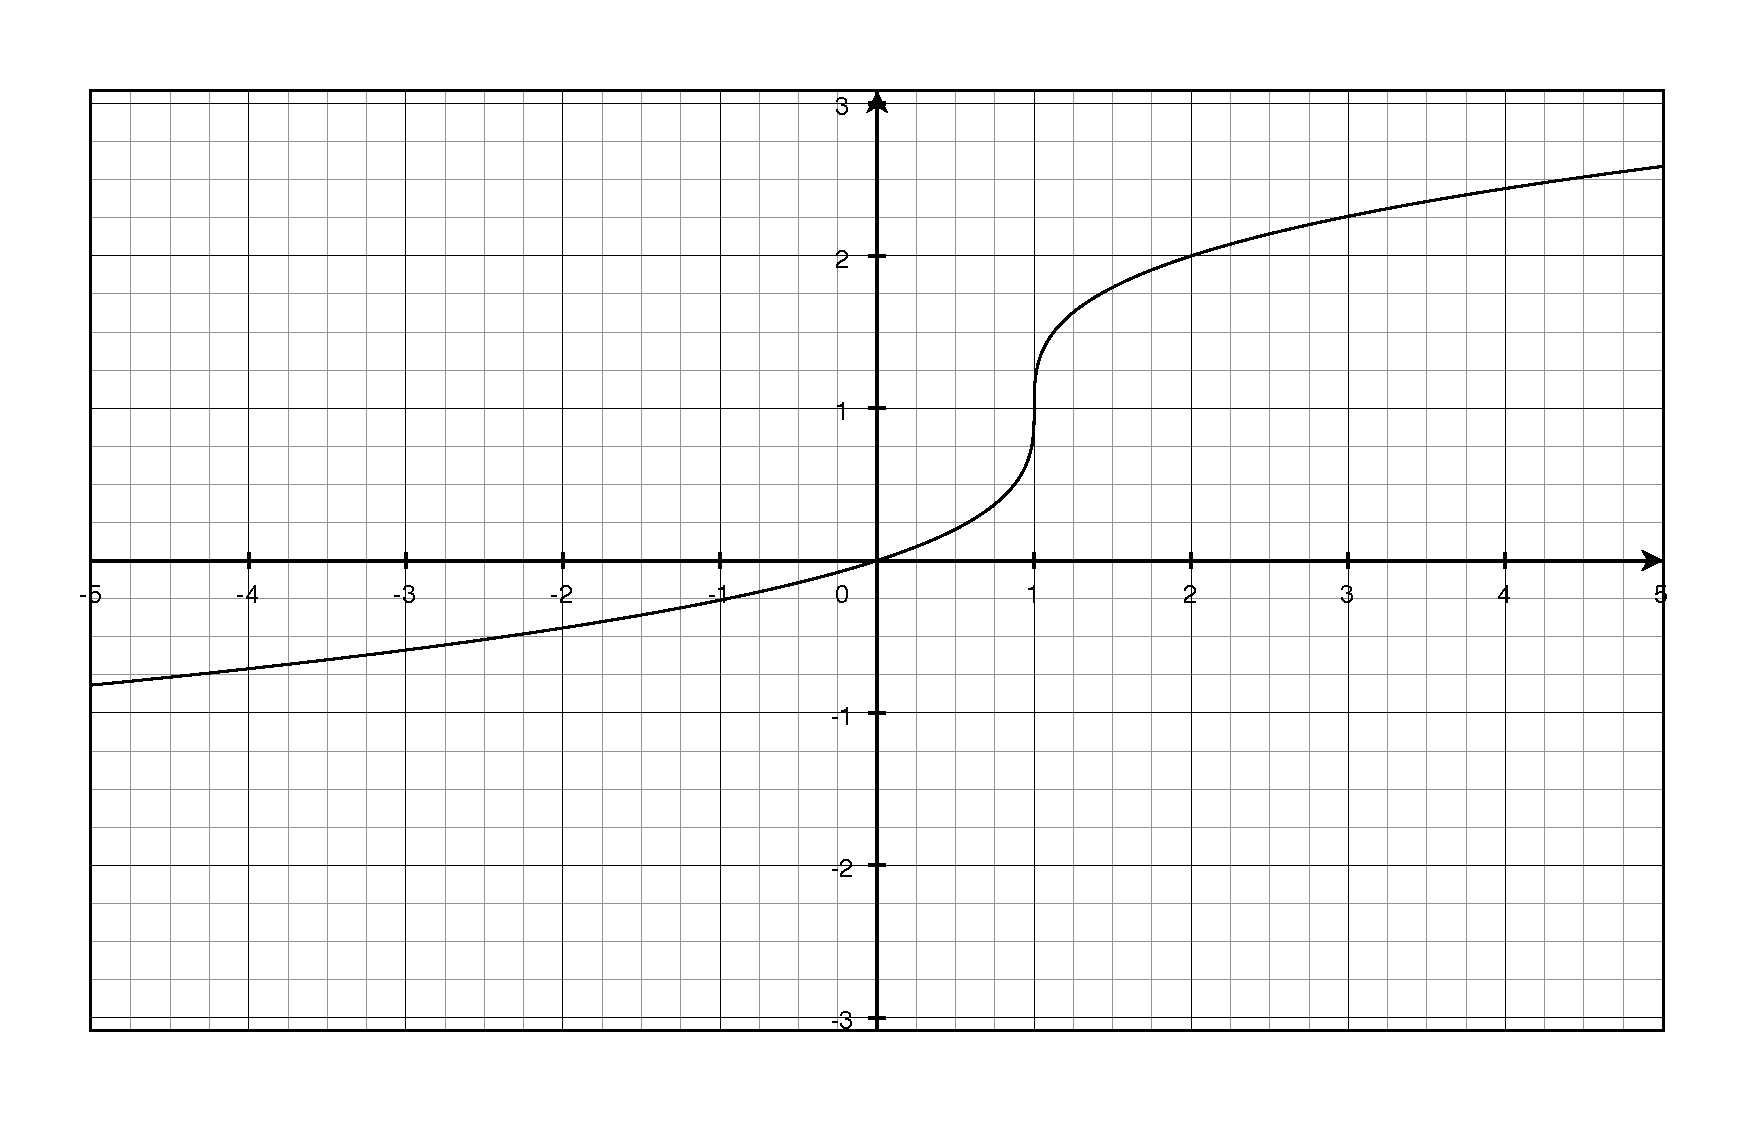
\includegraphics[scale=.3]{question7.eps}
%   \caption*{question 7}
% \end{figure}

% \begin{tabular}{cc}
%   \toprule
%   period & amplitude \\
%   \midrule
%     $\pi$ & $2$ \\
%   \bottomrule
% \end{tabular}

\printanswers
\excludecomment{comment}

\ifprintanswers 
  \usepackage{2in1, lscape} 
\fi

\author{}
\date{\today}
\title{Math 142 \\ Homework Two}

\begin{document}

  \maketitle

  \section{Homework}
  Section 5.2: 1-10, 15-22, 27-30, 45-66, 71-78, 80-81

  % \section{Extra Credit}
  % TO DO

  \ifprintanswers
    \section{Section 5.2}
    \begin{description}

      \item[1]
        Moving counterclockwise from $(1, 0)$:
        \begin{align*}
          \sin t &= 0, \frac{\sqrt{2}}{2}, 1, \frac{\sqrt{2}}{2}, 0, - \frac{\sqrt{2}}{2}, -1, - \frac{\sqrt{2}}{2} \\
          \cos t &= 1, \frac{\sqrt{2}}{2}, 0, - \frac{\sqrt{2}}{2}, -1, - \frac{\sqrt{2}}{2}, 0, \frac{\sqrt{2}}{2} \\
        \end{align*}

      \item[2]
        Moving counterclockwise from $(1, 0)$:
        \begin{align*}
          \sin t &= 0, \frac{1}{2}, \frac{\sqrt{3}}{2}, 1, \frac{\sqrt{3}}{2}, \frac{1}{2}, 0, -\frac{1}{2},
            -\frac{\sqrt{3}}{2}, -1, - \frac{\sqrt{3}}{2}, - \frac{1}{2} \\
          \cos t &= 1, \frac{\sqrt{3}}{2}, \frac{1}{2}, 0, - \frac{1}{2}, - \frac{\sqrt{3}}{2}, -1, - \frac{\sqrt{3}}{2}
              -\frac{1}{2}, 0, \frac{1}{2}, \frac{\sqrt{3}}{2} \\
        \end{align*}

      \item[3]
        \begin{align*}
          \sin \frac{2 \pi}{3} &= \frac{\sqrt{3}}{2} \\
          \cos \frac{2 \pi}{3} &= - \frac{1}{2} \\
          \tan \frac{2 \pi}{3} &= - \sqrt{3} \\
        \end{align*}

      \item[4]
        \begin{align*}
          \sin \frac{5 \pi}{6} &= \frac{1}{2} \\
          \cos \frac{5 \pi}{6} &= - \frac{\sqrt{3}}{2} \\
          \tan \frac{5 \pi}{6} &= - \frac{\sqrt{3}}{3} \\
        \end{align*}

      \item[5]
        \begin{align*}
          \sin \frac{7 \pi}{6}                 &= - \frac{1}{2} \\
          \sin \left( - \frac{\pi}{6} \right)  &= - \frac{1}{2} \\
          \sin \left( \frac{11 \pi}{6} \right) &= - \frac{1}{2} \\
        \end{align*}

      \item[6]
        \begin{align*}
          \cos \frac{5 \pi}{3}                  &= \frac{1}{2} \\
          \cos \left( - \frac{5 \pi}{3} \right) &= \frac{1}{2} \\
          \cos \frac{7 \pi}{3}                  &= \frac{1}{2} \\
        \end{align*}

      \item[7]
        \begin{align*}
          \cos \frac{3 \pi}{4} & = - \frac{\sqrt{2}}{2} \\
          \cos \frac{5 \pi}{4} & = - \frac{\sqrt{2}}{2} \\
          \cos \frac{7 \pi}{4} & = \frac{\sqrt{2}}{2} \\
        \end{align*}

      \item[8]
        \begin{align*}
          \sin \frac{3 \pi}{4} & = \frac{\sqrt{2}}{2} \\
          \sin \frac{5 \pi}{4} & = - \frac{\sqrt{2}}{2} \\
          \sin \frac{7 \pi}{4} & = - \frac{\sqrt{2}}{2} \\
        \end{align*}

      \item[9]
        \begin{align*}
          \sin \frac{7 \pi}{3} & = \frac{\sqrt{3}}{2} \\
          \csc \frac{7 \pi}{3} & = \frac{2 \sqrt{3}}{3} \\
          \cot \frac{7 \pi}{3} & = \frac{\sqrt{3}}{3} \\
        \end{align*}

      \item[10]
        \begin{align*}
          \cos \left( - \frac{\pi}{3} \right) & = \frac{1}{2} \\
          \sec \left( - \frac{\pi}{3} \right) & = 2 \\
          \tan \left( - \frac{\pi}{3} \right) & = - \sqrt{3} \\
        \end{align*}

      % \item[11]
      %   \begin{align*}
      %     \sin \left( - \frac{\pi}{2} \right) & = -1 \\
      %     \cos \left( - \frac{\pi}{2} \right) & = 0 \\
      %     \cot \left( - \frac{\pi}{2} \right) & = 0 \\
      %   \end{align*}

      % \item[12]
      %   \begin{align*}
      %     \sin \left( - \frac{3 \pi}{2} \right) & = 1 \\
      %     \cos \left( - \frac{3 \pi}{2} \right) & = 0 \\
      %     \cot \left( - \frac{3 \pi}{2} \right) & = 0 \\
      %   \end{align*}

      % \item[13]
      %   \begin{align*}
      %     \sec \frac{11 \pi}{3}               & = 2 \\
      %     \csc \frac{11 \pi}{3}               & = - \frac{2 \sqrt{3}}{3} \\
      %     \sec \left( - \frac{\pi}{3} \right) & = 2 \\
      %   \end{align*}

      % \item[14]
      %   \begin{align*}
      %     \cos \frac{7 \pi}{6} & = - \frac{\sqrt{3}}{2} \\
      %     \sec \frac{7 \pi}{6} & = - \frac{2 \sqrt{3}}{3} \\
      %     \csc \frac{7 \pi}{6} & = - 2 \\
      %   \end{align*}

      \item[15]
        \begin{align*}
          \tan \frac{5 \pi}{6}  & = - \frac{\sqrt{3}}{3} \\
          \tan \frac{7 \pi}{6}  & = \frac{\sqrt{3}}{3} \\
          \tan \frac{11 \pi}{6} & = - \frac{\sqrt{3}}{3} \\
        \end{align*}

      \item[16]
        \begin{align*}
          \cot \left( - \frac{\pi}{3} \right) & = - \frac{\sqrt{3}}{3} \\
          \cot \frac{2 \pi}{3}                & = - \frac{\sqrt{3}}{3} \\
          \cot \frac{5 \pi}{3}                & = - \frac{\sqrt{3}}{3} \\
        \end{align*}

      \item[17]
        \begin{align*}
          \cos \left( - \frac{\pi}{4} \right) & = \frac{\sqrt{2}}{2} \\
          \csc \left( - \frac{\pi}{4} \right) & = \sqrt{2} \\
          \cot \left( - \frac{\pi}{4} \right) & = 1 \\
        \end{align*}

      \item[18]
        \begin{align*}
          \sin \frac{5 \pi}{4} & = - \frac{\sqrt{2}}{2} \\
          \sec \frac{5 \pi}{4} & = - \sqrt{2} \\
          \tan \frac{5 \pi}{4} & = 1 \\
        \end{align*}

      \item[19]
        \begin{align*}
          \csc \left( - \frac{\pi}{2} \right) & = -1 \\
          \csc \frac{\pi}{2}                  & = 1 \\
          \csc \frac{3 \pi}{2}                & = - 1 \\
        \end{align*}

      \item[20]
        \begin{align*}
          \sec (- \pi) & = -1 \\
          \sec \pi     & = -1 \\
          \sec 4 \pi   & = 1 \\
        \end{align*}

      \item[21]
        \begin{align*}
          \sec 13 \pi & = -1 \\
          \cos 14 \pi & = 1 \\
          \tan 15 \pi & = 0 \\
        \end{align*}

      \item[22]
        \begin{align*}
          \sin \left( \frac{25 \pi}{2} \right) & = 1 \\
          \cos \left( \frac{25 \pi}{2} \right) & = 0 \\
          \cot \left( \frac{25 \pi}{2} \right) & = 0 \\
        \end{align*}

      \item[27]
        \begin{align*}
          \sin t & = \frac{4}{5} \\
          \cos t & = \frac{3}{5} \\
          \tan t & = \frac{4}{3} \\
        \end{align*}

      \item[28]
        \begin{align*}
          \sin t & = \frac{4}{5} \\
          \cos t & = - \frac{3}{5} \\
          \tan t & = - \frac{4}{3} \\
        \end{align*}

      \item[29]
        \begin{align*}
          \sin t & = - \frac{\sqrt{11}}{4} \\
          \cos t & = \frac{\sqrt{5}}{4} \\
          \tan t & = - \sqrt{\frac{11}{5}} \\
        \end{align*}

      \item[30]
        \begin{align*}
          \sin t & = - \frac{2 \sqrt{2}}{3} \\
          \cos t & = - \frac{1}{3} \\
          \tan t & = 2 \sqrt{2} \\
        \end{align*}

      \item[45]
        In quadrant II, $\sin t$ is positive and $\cos t$ is negative, so $\sin t \cos t$ is \fbox{negative}.

      \item[46]
        \[
          \tan t \sec t = \frac{\sin t}{\cos t} \cdot \frac{1}{\cos t} = \frac{\sin t}{\cos^2 t}
        \]

        Since $\cos^2 t$ is always positive and $\sin t$ is negative in quadrant IV, the result is \fbox{negative}.

      \item[47]
        \[
          \frac{\tan t \sin t}{\cot t} = \tan^2 t \sin t
        \]

        Since $\tan^2 t$ is always positive and $\sin t$ is negative in quadrant III, the result is \fbox{negative}.

      \item[48]
        \[
          \cos t \sec t = \cos t \cdot \frac{1}{\cos t} = 1
        \]

        The value is always 1 which is \fbox{positive}.

      \item[49] $\sin t > 0$ in quadrants I and II and $\cos t < 0$ in quadrants II and III, so the value must be in
        \fbox{quadrant II}.

      \item[50] $\tan t > 0$ in quadrants I and III and $\sin t < 0$ in quadrants III and IV, so the value must be in
        \fbox{quadrant III}.

      \item[51] $\csc t = \frac{1}{\sin t} > 0$ in quadrants I and II and $\sec t = \frac{1}{\cos t} < 0$ in quadrants
        II and III, so the value must be in \fbox{quadrant II}.

      \item[52] $\cos t < 0$ in quadrants II and III and $\cot t < 0$ in quadrants II and IV, so the value must be in
        \fbox{quadrant II}.

      \item[53] In quadrant II: $\cos t = \boxed{ - \sqrt{1 - \sin^2 t} }$

      \item[54] In quadrant IV: $\sin t = \boxed{ - \sqrt{1 - \cos^2 t} }$

      \item[55] 
        \begin{align*}
          \tan^2 t + 1 & = \sec^2 t \\
          \tan^2 t     & = \sec^2 t - 1 \\
          \tan^2 t     & = \frac{1}{\cos^2 t} - 1 \\
          \tan^2 t     & = \frac{1 - \cos^2 t}{\cos^2 t} \\
          \tan^2 t     & = \frac{\sin^2 t}{1 - \sin^2 t} \\
          \tan t       & = \pm \sqrt{ \frac{\sin^2 t}{1 - \sin^2 t} } \\
        \end{align*}

        In quadrant IV, $\tan t = \boxed{ - \sqrt{ \frac{\sin^2 t}{1 - \sin^2 t} } }$

      \item[56] 
        \begin{align*}
          \tan^2 t + 1 & = \sec^2 t \\
          \tan^2 t     & = \sec^2 t - 1 \\
          \tan^2 t     & = \frac{1}{\cos^2 t} - 1 \\
          \tan^2 t     & = \frac{1 - \cos^2 t}{\cos^2 t} \\
          \tan t     & = \pm \sqrt{ \frac{1 - \cos^2 t}{\cos^2 t} } \\
        \end{align*}

        $\tan t$ is positive in quadrant III and $\frac{1}{\cos^2 t} \geq 1$ everywhere.  
        
        So in quadrant III: $\tan t = \boxed{ \sqrt{ \frac{1 - \cos^2 t}{\cos^2 t} } }$

      \item[57] 
        \begin{align*}
          \sec^2 t & = \tan^2 t + 1 \\
          \sec t   & = \pm \sqrt{\tan^2 t + 1} \\
        \end{align*}

        In quadrant II, $\sec t = \boxed{ - \sqrt{\tan^2 t + 1} }$ 

      \item[58] 
        \begin{align*}
          \csc^2 t & = \cot^2 t + 1 \\
          \csc t   & = \pm \sqrt{\cot^2 t + 1} \\
        \end{align*}

        In quadrant III, $\csc t = \boxed{ - \sqrt{\cot^2 t + 1} }$ 

      \item[59] 
        \begin{align*}
          \sec^2 t & = \tan^2 t + 1 \\
          \tan^2 t & = \sec^2 t - 1 \\
          \tan t   & = \pm \sqrt{ \sec^2 t - 1 } \\
        \end{align*}

        In quadrant III, $t = \boxed{\tan \sqrt{ \sec^2 t - 1 }}$ 

      \item[60] 
        \begin{align*}
          \sin^2 t + \cos^2 t           & = 1 \\
          \sin^2 t + \frac{1}{\sec^2 t} & = 1 \\
          \sin^2 t                      & = 1 - \frac{1}{\sec^2 t} \\
          \sin t                        & = \pm \sqrt{ 1 - \frac{1}{\sec^2 t} } \\
        \end{align*}

        In quadrant IV, $\sin t = \boxed{ - \sqrt{ 1 - \frac{1}{\sec^2 t} } }$ 

      \item[61] 
        \begin{align*}
          \tan^2 t & = 1 + \sec^2 t \\
                   & = 1 + \frac{1}{\cos^2 t} \\
                   & = 1 + \frac{1}{1 - \sin^2 t} \\
                   & = \boxed{ \frac{2 - \sin^2 t}{1 - \sin^2 t} } \\
        \end{align*}

      \item[62] 
        \begin{align*}
          \tan^2 t + 1                  & = \sec^2 t \\
          \frac{\sin^2 t}{\cos^2 t} + 1 & = \sec^2 t \\
          \sec^2 t \sin^2 t             & = \frac{1}{\cos^2 t} - 1 \\
          \sec^2 t \sin^2 t             & = \boxed{ \frac{1 - \cos^2 t}{\cos^2 t} } \\
        \end{align*}

      \item[63]
        \begin{tabular}[H]{cccccc}
          \toprule
          $\sin t$      & $\cos t$        & $\tan t$        & $\csc t$      & $\sec t$        & $\cot t$ \\
          \midrule
          $\frac{3}{5}$ & $- \frac{4}{5}$ & $- \frac{3}{4}$ & $\frac{5}{3}$ & $- \frac{5}{4}$ & $- \frac{4}{3}$ \\
          \bottomrule
        \end{tabular}

      \item[64]
        \begin{tabular}[H]{cccccc}
          \toprule
          $\sin t$        & $\cos t$        & $\tan t$      & $\csc t$        & $\sec t$        & $\cot t$ \\
          \midrule
          $- \frac{3}{5}$ & $- \frac{4}{5}$ & $\frac{3}{4}$ & $- \frac{5}{3}$ & $- \frac{5}{4}$ & $\frac{4}{3}$ \\
          \bottomrule
        \end{tabular}

      \item[65]
        \begin{tabular}[H]{cccccc}
          \toprule
          $\sin t$                 & $\cos t$      & $\tan t$       & $\csc t$                 & $\sec t$ & $\cot t$ \\
          \midrule
          $- \frac{2 \sqrt{2}}{3}$ & $\frac{1}{3}$ & $- 2 \sqrt{2}$ & $- \frac{3 \sqrt{2}}{4}$ & $3$      & $- \frac{\sqrt{2}}{4}$ \\
          \bottomrule
        \end{tabular}

      \item[66]
        \begin{tabular}[H]{cccccc}
          \toprule
          $\sin t$                & $\cos t$                  & $\tan t$      & $\csc t$     & $\sec t$               & $\cot t$ \\
          \midrule
          $-\frac{\sqrt{17}}{17}$ & $-\frac{4 \sqrt{17}}{17}$ & $\frac{1}{4}$ & $-\sqrt{17}$ & $-\frac{\sqrt{17}}{4}$ & $4$ \\
          \bottomrule
        \end{tabular}

      % \item[67]
      %   If $\cos t > 0$ and $\tan t < 0$, the point is in quadrant IV

      %   \begin{tabular}[H]{cccccc}
      %     \toprule
      %     $\sin t$       & $\cos t$      & $\tan t$       & $\csc t$       & $\sec t$      & $\cot t$ \\
      %     \midrule
      %     $-\frac{3}{5}$ & $\frac{4}{5}$ & $-\frac{3}{4}$ & $-\frac{5}{3}$ & $\frac{5}{4}$ & $\frac{4}{3}$ \\
      %     \bottomrule
      %   \end{tabular}

      % \item[68]
      %   If $\sec t > 0$ and $\sin t < 0$, the point is in quadrant IV

      %   \begin{tabular}[H]{cccccc}
      %     \toprule
      %     $\sin t$              & $\cos t$      & $\tan t$    & $\csc t$                & $\sec t$ & $\cot t$ \\
      %     \midrule
      %     $-\frac{\sqrt{3}}{2}$ & $\frac{1}{2}$ & $-\sqrt{3}$ & $-\frac{2 \sqrt{3}}{3}$ & $2$      & $-\frac{\sqrt{3}}{3}$ \\
      %     \bottomrule
      %   \end{tabular}

      % \item[69]
      %   If $\sin t < 0$ and $\sec t < 0$, the point is in quadrant III

      %   \begin{tabular}[H]{cccccc}
      %     \toprule
      %     $\sin t$       & $\cos t$              & $\tan t$                & $\csc t$ & $\sec t$                 & $\cot t$ \\
      %     \midrule
      %     $-\frac{1}{4}$ & $\frac{\sqrt{15}}{4}$ & $-\frac{\sqrt{15}}{15}$ & $-4$     & $\frac{4 \sqrt{15}}{15}$ & $-\sqrt{15}$ \\
      %     \bottomrule
      %   \end{tabular}

      % \item[70]
      %   If $\tan t < 0$ and $\csc t > 0$, the point is in quadrant II

      %   \begin{tabular}[H]{cccccc}
      %     \toprule
      %     $\sin t$                 & $\cos t$                & $\tan t$ & $\csc t$              & $\sec t$     & $\cot t$ \\
      %     \midrule
      %     $\frac{4 \sqrt{17}}{17}$ & $-\frac{\sqrt{17}}{17}$ & $-4$     & $\frac{\sqrt{17}}{4}$ & $-\sqrt{17}$ & $-\frac{1}{4}$ \\
      %     \bottomrule
      %   \end{tabular}

      \item[71]
        \begin{align*}
          f(-x) & = (-x)^2 \sin(-x) \\
                & = - x^2 \sin x \\
                & = - f(x) \\
        \end{align*}

        \boxed{odd}

      \item[72]
        \begin{align*}
          f(-x) & = (-x)^2 \cos(-2x) \\
                & = x^2 \cos 2x \\
                & = f(x) \\
        \end{align*}

        \boxed{even}

      \item[73]
        \begin{align*}
          f(-x) & = \sin (-x) \cos (-x) \\
                & = - \sin x \cos x \\
                & = -f(x) \\
        \end{align*}

        \boxed{odd}

      \item[74]
        \begin{align*}
          f(-x) & = \sin (-x) + \cos (-x) \\
                & = - \sin x + \cos x \\
        \end{align*}

        \boxed{neither}

      \item[75]
        \begin{align*}
          f(-x) & = | -x | \cos (-x) \\
                & = x \cos x \\
                & = f(x) \\
        \end{align*}
        \boxed{even}

      \item[76]
        \begin{align*}
          f(-x) & = (-x)^3 \sin^3 (-x) \\
                & = - x^3 \sin^3 x \\
                & = - f(x) \\
        \end{align*}
        \boxed{odd}

      \item[77]
        \begin{align*}
          f(-x) & = (-x)^3 + \cos x \\
                & = - x^3 + \cos x \\
        \end{align*}
        \boxed{neither}

      \item[78]
        \begin{align*}
          f(x) & = \cos (\sin (-x)) \\
               & = \cos (- \sin x) \\
               & = \cos (\sin x) \\
               & = f(x) \\
        \end{align*}
        \boxed{even}

      \item[80]
        \begin{tabular}[H]{lr}
          \toprule
          6:00 am  & 87 \\
          10:30 am & 83 \\
          noon     & 80 \\
          8:00 pm  & 74 \\
          \bottomrule
        \end{tabular}

      \item[81]
        \begin{align*}
          I(0.1) & \approx \boxed{ 0.4987 } \\
          I(0.5) & \approx \boxed{ -0.1712 } \\
        \end{align*}
    \end{description}
  \else
    \vspace{1 cm}
    \begin{quote}
      \begin{em}
        TO DO
      \end{em}
    \end{quote}
    \hspace{1 cm} --Shunryu Suzuki
  \fi

\end{document}

